% 15-20 pages

\documentclass[11pt,a4paper]{article}

\usepackage[T1]{fontenc}
\usepackage[a4paper,margin=2.5cm]{geometry}
\usepackage{xcolor}

\usepackage{graphicx}
\usepackage{float}
\usepackage{placeins}

\graphicspath{{../images/}}

\definecolor{titleblue}{HTML}{1F4E79}

\usepackage{csquotes}
\usepackage[backend=biber, style=numeric, sorting=none ]{biblatex}
\addbibresource{references.bib}

\addbibresource{references.bib}

\usepackage{xurl}
\usepackage[hidelinks, breaklinks=true]{hyperref}


\begin{document}

\begin{titlepage}
	\centering
	
	\vspace*{2cm}
	
	{\large
		Data Engineer Programme\\
		Liora
		\par}
	
	\vspace{2.5cm}
	
	{\color{titleblue}\rule{\textwidth}{1.5pt}}
	
	\vspace{0.8cm}
	
	{\Huge\bfseries
		Job Market
		\par}
	
	\vspace{0.5cm}
	
	{\Large
		Design and Implementation of an End-to-End\\
		Data Engineering Pipeline
		\par}
	
	\vspace{0.8cm}
	
	{\color{titleblue}\rule{\textwidth}{1.5pt}}
	
	\vfill
	
	\begin{tabular}{rl}
		\textbf{Project team:} &
		TODO\\[0.5cm]
		
		\textbf{Programme:} & Data Engineer \\[0.2cm]
		\textbf{Organisation:} & Liora \\[0.2cm]
		\textbf{Project period:} & 2026 \\[0.2cm]
		\textbf{Report date:} & \today
	\end{tabular}
	
	\vfill
	
	{\small
		Project Report
		\par}
	
\end{titlepage}

\tableofcontents
\listoffigures


The job advertisements are retrieved through the Arbeitsagentur Jobsuche interface \cite{arbeitsagentur-api}.

FastAPI provides typed request handling and automatically generated OpenAPI documentation \cite{fastapi-docs}.

The dashboard is implemented with Plotly Dash \cite{dash-docs}.

PostgreSQL is used as the authoritative structured data store \cite{postgresql-docs}, while SQLAlchemy manages database connections and SQL execution \cite{sqlalchemy-docs}.
The application services are defined and started as a multi-container application using Docker Compose \cite{docker-compose-docs}.
The ETL workflow is scheduled through Apache Airflow \cite{airflow-docs}.


Multiple sources can be cited together:

Operational metrics are collected with Prometheus and visualised in Grafana \cite{prometheus-docs,grafana-docs}.


For the Pushgateway decision:

The ETL process is a short-lived batch job and therefore cannot be
scraped continuously. It publishes its metrics through Pushgateway,
which acts as an intermediary for jobs of this kind
\cite{prometheus-pushgateway}.


For geocoding:

Missing coordinates are retrieved using the Nominatim search API
\cite{nominatim-api}. Requests are rate-limited to comply with the
public service's usage policy \cite{nominatim-policy}.

\newpage


\section{Introduction}

\subsection{Project Context}
%Explain the motivation: job advertisements contain useful information about employers, locations, demanded occupations, home-office opportunities, and market composition.

\subsection{Project Objectives}

Figure~\ref{fig:project-overview} presents the overall architecture of
the Job Market system. The architecture is divided into an ingestion
layer and a runtime layer.
	
\begin{figure}[htbp]
	\centering
	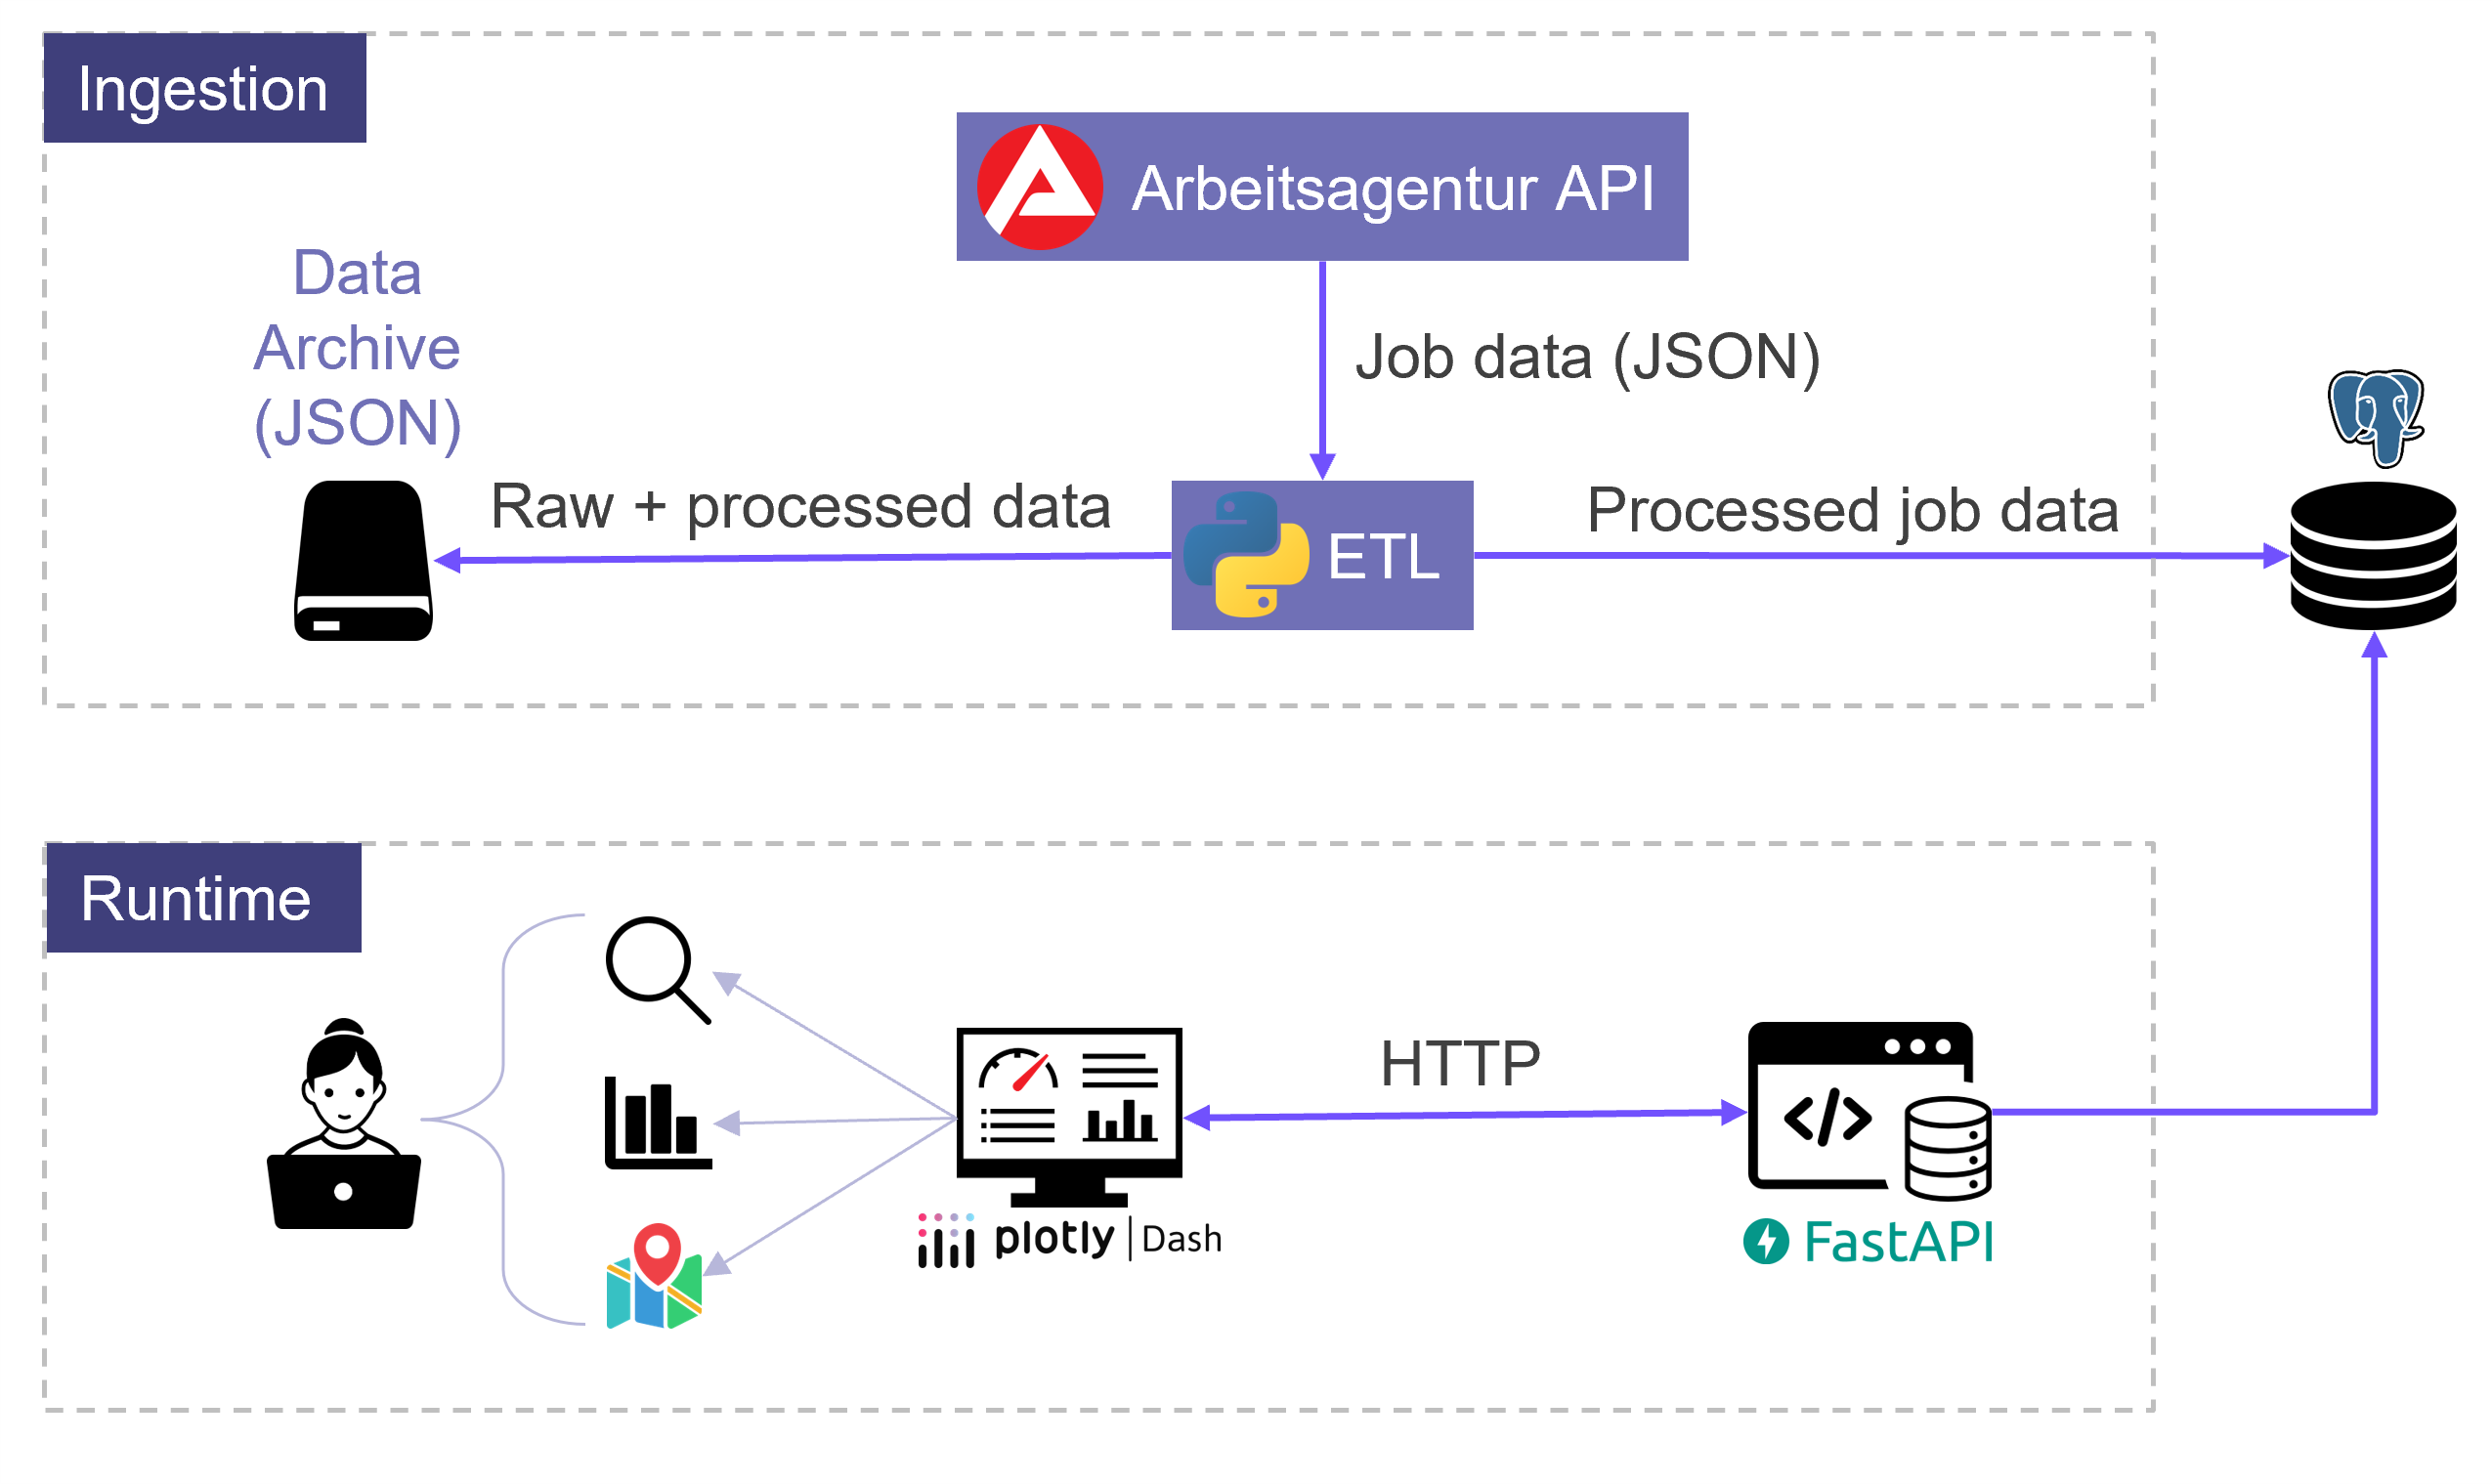
\includegraphics[
	width=\textwidth,
	height=0.72\textheight,
	keepaspectratio
	]{project-overview.png}
	\caption{Overall architecture of the Job Market system.}
	\label{fig:project-overview}
\end{figure}

State what the system is intended to accomplish:

	retrieve German job advertisements;
	preserve raw extraction results;
	transform and enrich the data;
	store structured records in PostgreSQL;
	make the data accessible through an API;
	provide an interactive dashboard;
	automate and monitor the pipeline.

\subsection{Scope and Limitations}
Clarify the boundaries:

only the Bundesagentur für Arbeit is currently used;
the project is focused on German job advertisements;
categories are rule-based;
the system is an educational prototype, not a production job portal;
no machine-learning component is included;
Elasticsearch is a possible future extension.

This section should be approximately 1–1.5 pages.


\section{System Architecture}

\subsection{Architectural Overview}
Introduce the main components:

Bundesagentur für Arbeit API;
ETL pipeline;
raw and processed JSON storage;
PostgreSQL;
FastAPI;
Dash;
Airflow;
Prometheus, Pushgateway, Alertmanager, and Grafana;
Docker Compose.

\subsection{Data Flow}
Describe the central flow:
Arbeitsagentur API
↓
Extract → Transform → Load
↓               ↓
JSON history     PostgreSQL
↓
FastAPI
↓
Dash

Also explain that monitoring data takes a separate path to Prometheus.

\subsection{Project Organisation}
Briefly explain the code structure under src/api, src/data, src/dashboard, src/monitoring, and src/tests.

Do not reproduce the complete directory tree. A compact table is enough.

Approximately 1.5–2 pages.


\section{Data Collection and ETL Pipeline}

The ingestion process is divided into the three conventional ETL stages
shown in Figure~\ref{fig:ingestion-pipeline}.

\begin{figure}[htbp]
	\centering
	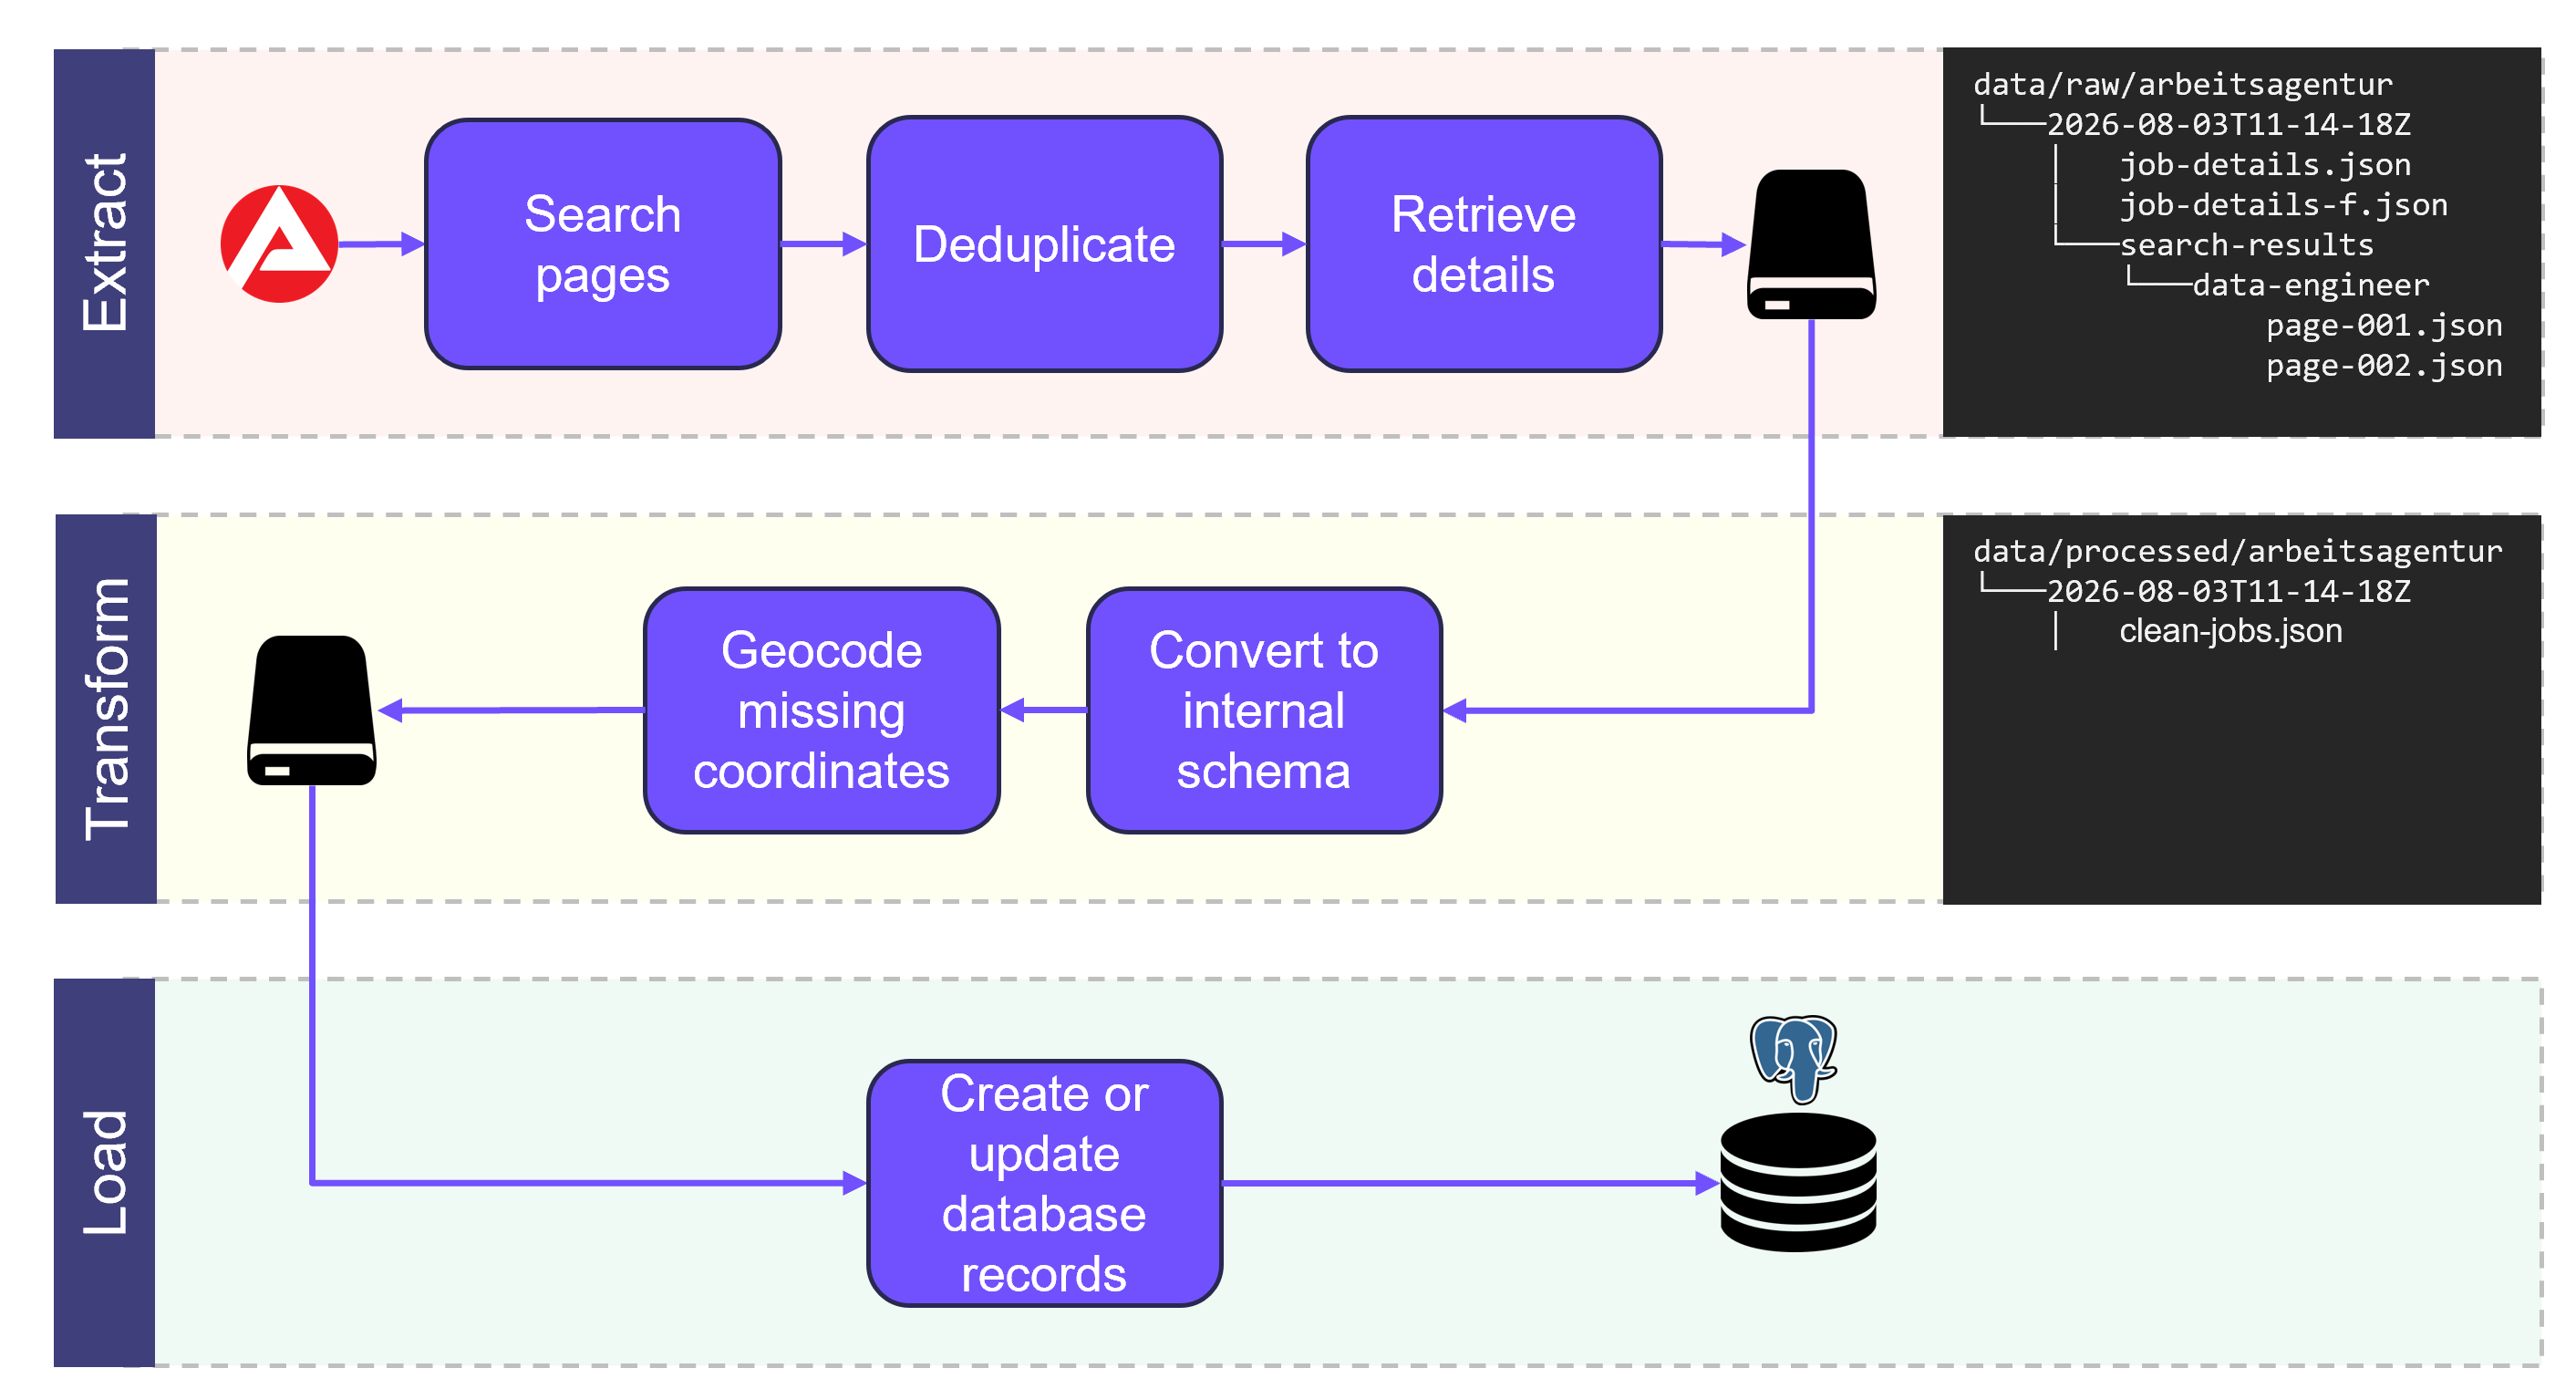
\includegraphics[
	width=\textwidth,
	height=0.75\textheight,
	keepaspectratio
	]{ingestion.png}
	\caption{Extract, transform, and load stages of the ingestion pipeline.}
	\label{fig:ingestion-pipeline}
\end{figure}
	

\subsection{Data Source}
Describe the Bundesagentur für Arbeit API:

search endpoint;
job-detail endpoint;
returned JSON data;
relevant fields;
practical limitations and possible request failures.

We should explain why it was chosen instead of pretending that all sources proposed in the assignment were implemented.

\subsection{Extraction}
%Describe extract_data.py and arbeitsagentur_client.py:

multiple search keywords;
paginated search results;
retrieval of full job details;
duplicate reference numbers;
storage of failed detail requests;
timestamped raw-data directories.

\subsection{Transformation}
%Describe transform_data.py:

mapping German API field names to the internal English schema;
handling missing or malformed structures;
conversion of nested locations;
creation of clean JSON output.

\subsection{Location Enrichment}
Explain the geocoding process:

coordinates supplied by the source are retained;
missing coordinates are requested from Nominatim;
rate limiting and retries;
in-memory caching;
failed geocoding attempts are counted.

\subsection{Job Classification}
Explain the broad categories:

Data Engineering;
Data Analysis;
AI / Machine Learning;
Backend Development;
Cloud / DevOps;
Other.

Also describe:

classification based on title and occupation;
keyword priority;
word-boundary handling for short keywords such as AI;
limitations of rule-based classification.	

\subsection{Loading and Update Strategy}
%Describe load_data.py:

schema creation;
insertion or updating of jobs;
handling of job locations;
reference number as the stable identifier;
PostgreSQL as the authoritative structured data store.

Approximately 3–3.5 pages. This should be one of the largest chapters because ETL is central to the assignment.


\section{Data Modelling and Storage}

\subsection{Storage Strategy}

The project uses a two-layer storage strategy. Raw API responses are preserved in timestamped JSON directories, forming a lightweight historical raw-data layer. This layer is data-lake-like in the sense that it retains source data in its original form, but a full data-lake infrastructure would introduce unnecessary storage, cataloguing, and operational complexity for a project with a single data source and a moderate data volume. The file-based archive makes individual extraction runs traceable and allows transformations to be reproduced without requiring additional infrastructure.

PostgreSQL was selected for the transformed data because job postings and locations form a clearly defined relational structure. The application frequently filters, joins, aggregates, and performs statistical queries over these records. PostgreSQL therefore provides referential integrity, indexing, transactions, and efficient SQL-based analysis, while integrating well with Python, SQLAlchemy, and FastAPI.

A document database such as MongoDB could store the original nested API responses conveniently, but this flexibility provides little advantage after transformation into the stable application schema. It would also move relationships and consistency checks into application code and make relational queries and aggregations less direct. Retaining raw JSON files and loading the structured result into PostgreSQL therefore provides the required flexibility without operating two database systems.

\subsection{Relational Data Model}

The transformed data is represented by two related tables. The \texttt{Job} table stores the attributes of a job posting and uses the reference number supplied by the source API as its primary key. The \texttt{JobLocation} table stores the associated geographical information. Its \texttt{reference\_number} column is a foreign key referring to the corresponding job.

Figure~\ref{fig:erd} shows the resulting relational data model. A job may have zero or more associated locations, whereas each location belongs to exactly one job.

\begin{figure}[htbp]
	\centering
	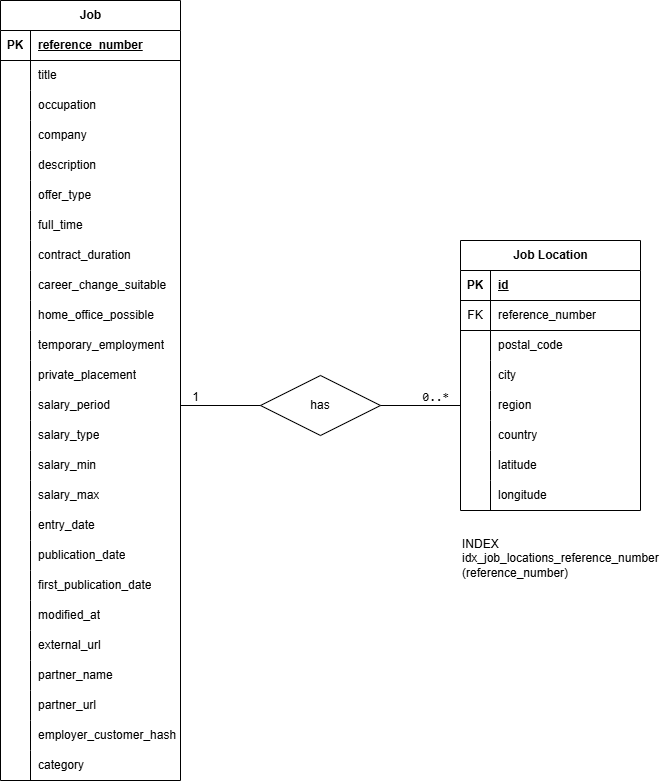
\includegraphics[width=0.72\textwidth, height=0.72\textheight, keepaspectratio]{erd.png}
	\caption{Entity--relationship diagram of the job-market database}
	\label{fig:erd}
\end{figure}

The separation of jobs and locations avoids repeating the complete job record when a posting is associated with multiple locations. The foreign-key constraint preserves referential integrity. An index on \texttt{JobLocation.reference\_number} supports efficient joins and location-based queries.

\subsection{Data Integrity and Query Performance}
Discuss:

primary and foreign keys;
%the index on job_locations.reference_number;
handling nullable API fields;
avoiding duplicate job records;
replacing or updating related locations.

Approximately 1.5–2 pages.


\section{Data Access and Visualisation}

\subsection{FastAPI Backend}
Explain why FastAPI was selected:

typed request and response models;
automatic OpenAPI documentation;
validation through Pydantic;
separation between application data and the user interface.

\subsection{Job API}
Describe the important endpoints:

%GET /health;
%GET /jobs;
%GET /jobs/{reference_number}.

Mention filtering by:

keyword;
city;
company;
home-office availability;
category;
pagination.

Include one small request-and-response example or a Swagger screenshot—not both in excessive detail.

\subsection{Statistics API}
Describe the endpoints for:

general overview;
top companies;
top locations;
home-office distribution;
job-category distribution.

\subsection{Dash Frontend}

The main dashboard view combines search controls, a paginated result
list, and an interactive map, as shown in
Figure~\ref{fig:job-search-interface}.

\begin{figure}[htbp]
	\centering
	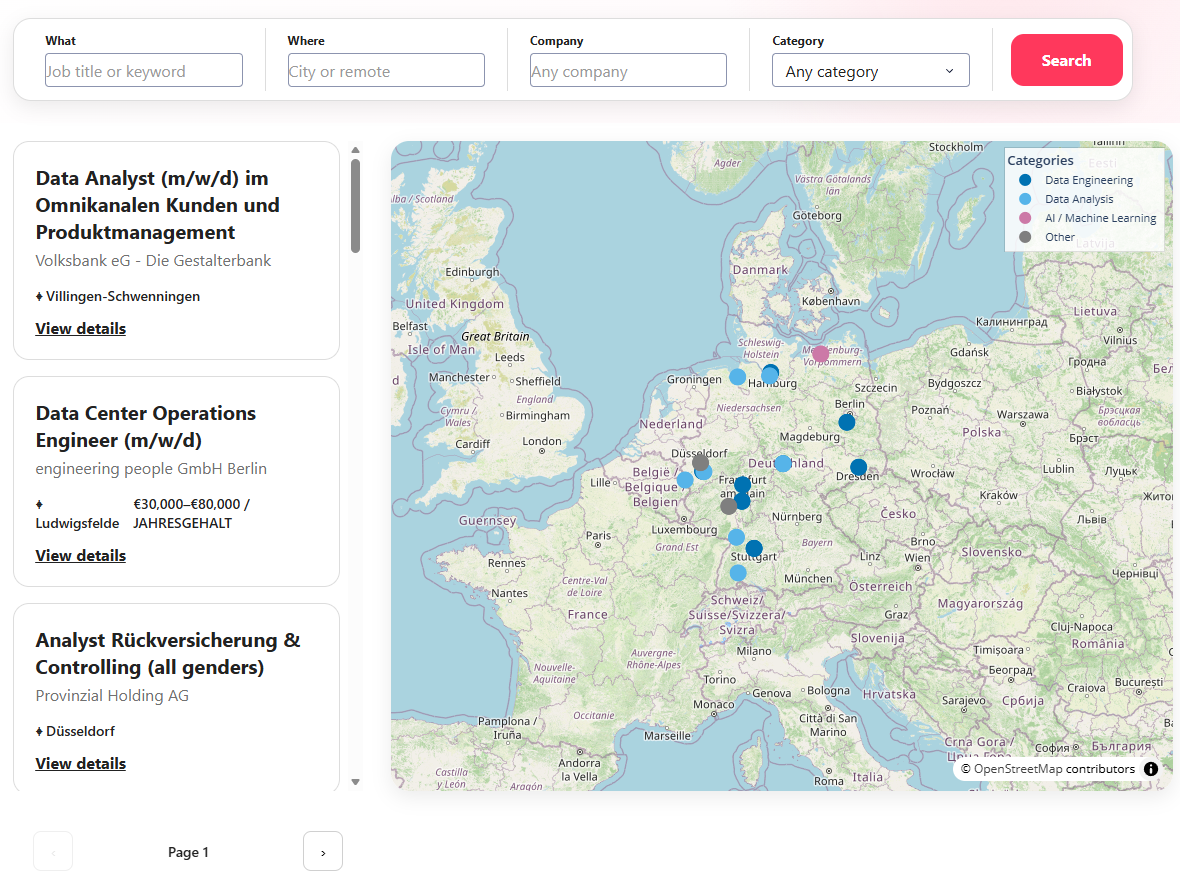
\includegraphics[
	width=\textwidth,
	height=0.75\textheight,
	keepaspectratio
	]{find-jobs-ui.png}
	\caption{Job search interface with filters, results, and an interactive map.}
	\label{fig:job-search-interface}
\end{figure}

	Explain the frontend features:
	
	search form;
	result list;
	job-detail view;
	interactive map;
	category-coloured markers;
	statistics page;
	database-unavailable notification.

\subsection{Visual Analytics}

The statistics view summarises the geographical distribution of jobs,
home-office availability, and the distribution of standardised job
categories (Figure~\ref{fig:statistics-interface}).

\begin{figure}[p]
	\centering
	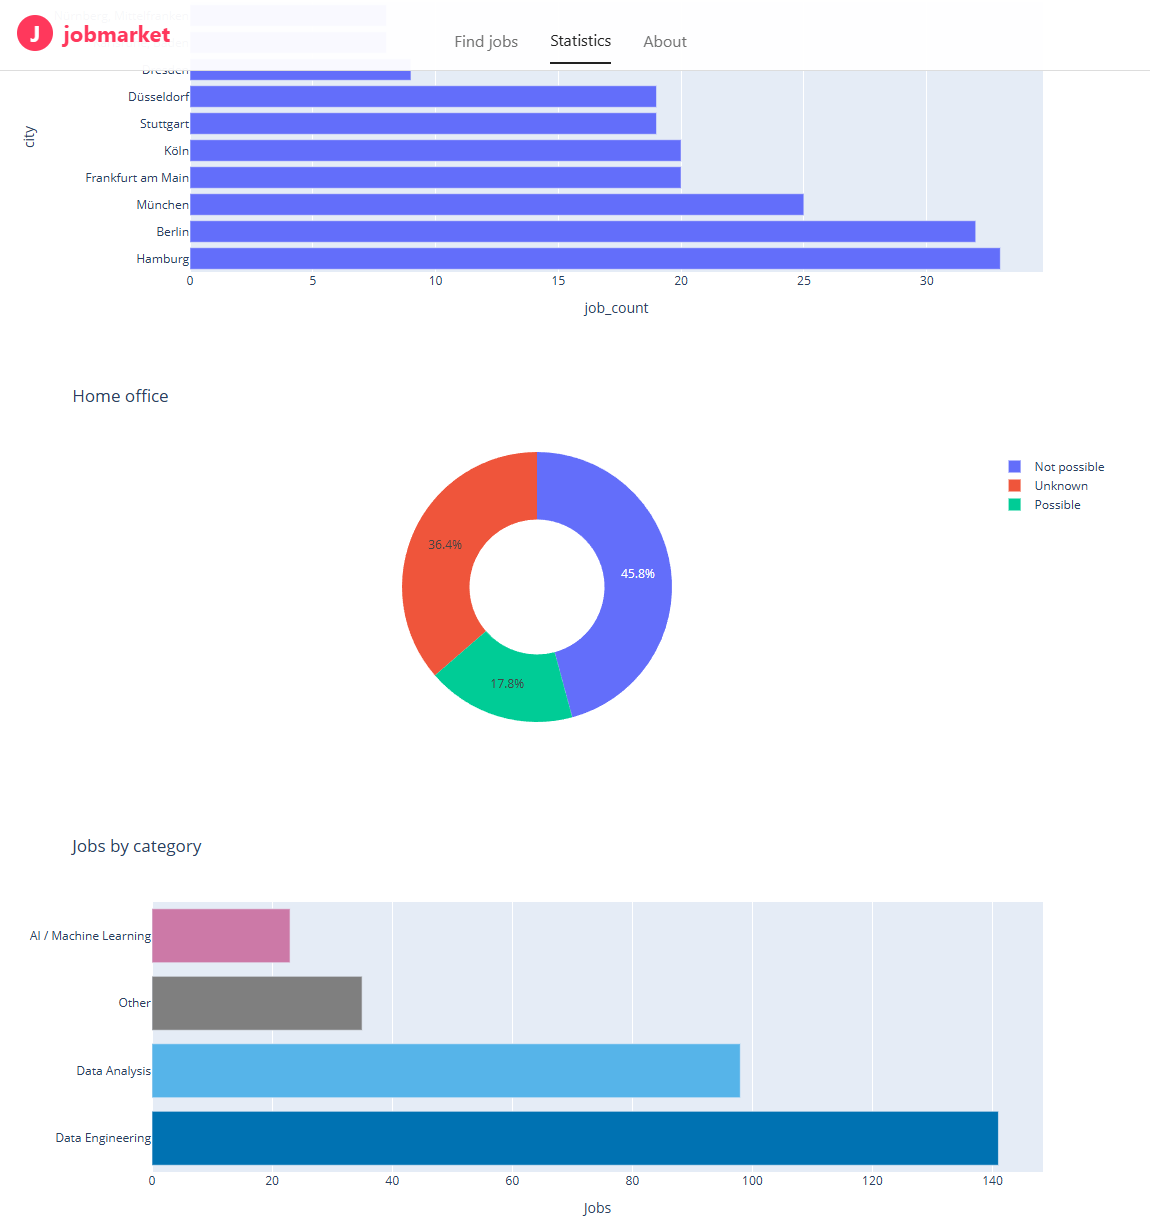
\includegraphics[
	width=0.9\textwidth,
	height=0.82\textheight,
	keepaspectratio
	]{statistics-ui.png}
	\caption{Statistical analysis of locations, home-office availability,
		and job categories.}
	\label{fig:statistics-interface}
\end{figure}
Explain what users can learn from:

company statistics;
location statistics;
home-office distribution;
category distribution;
the geographical map.

This should explain the meaning of the visualisations, not just state that charts exist.


\section{Deployment and Automation}

\subsection{Containerisation}
Describe the shared application image and the separate service containers.

\subsection{Docker Compose Deployment}

Figure~\ref{fig:docker-deployment} shows the services started through
Docker Compose and the principal communication paths between them.

\begin{figure}[htbp]
	\centering
	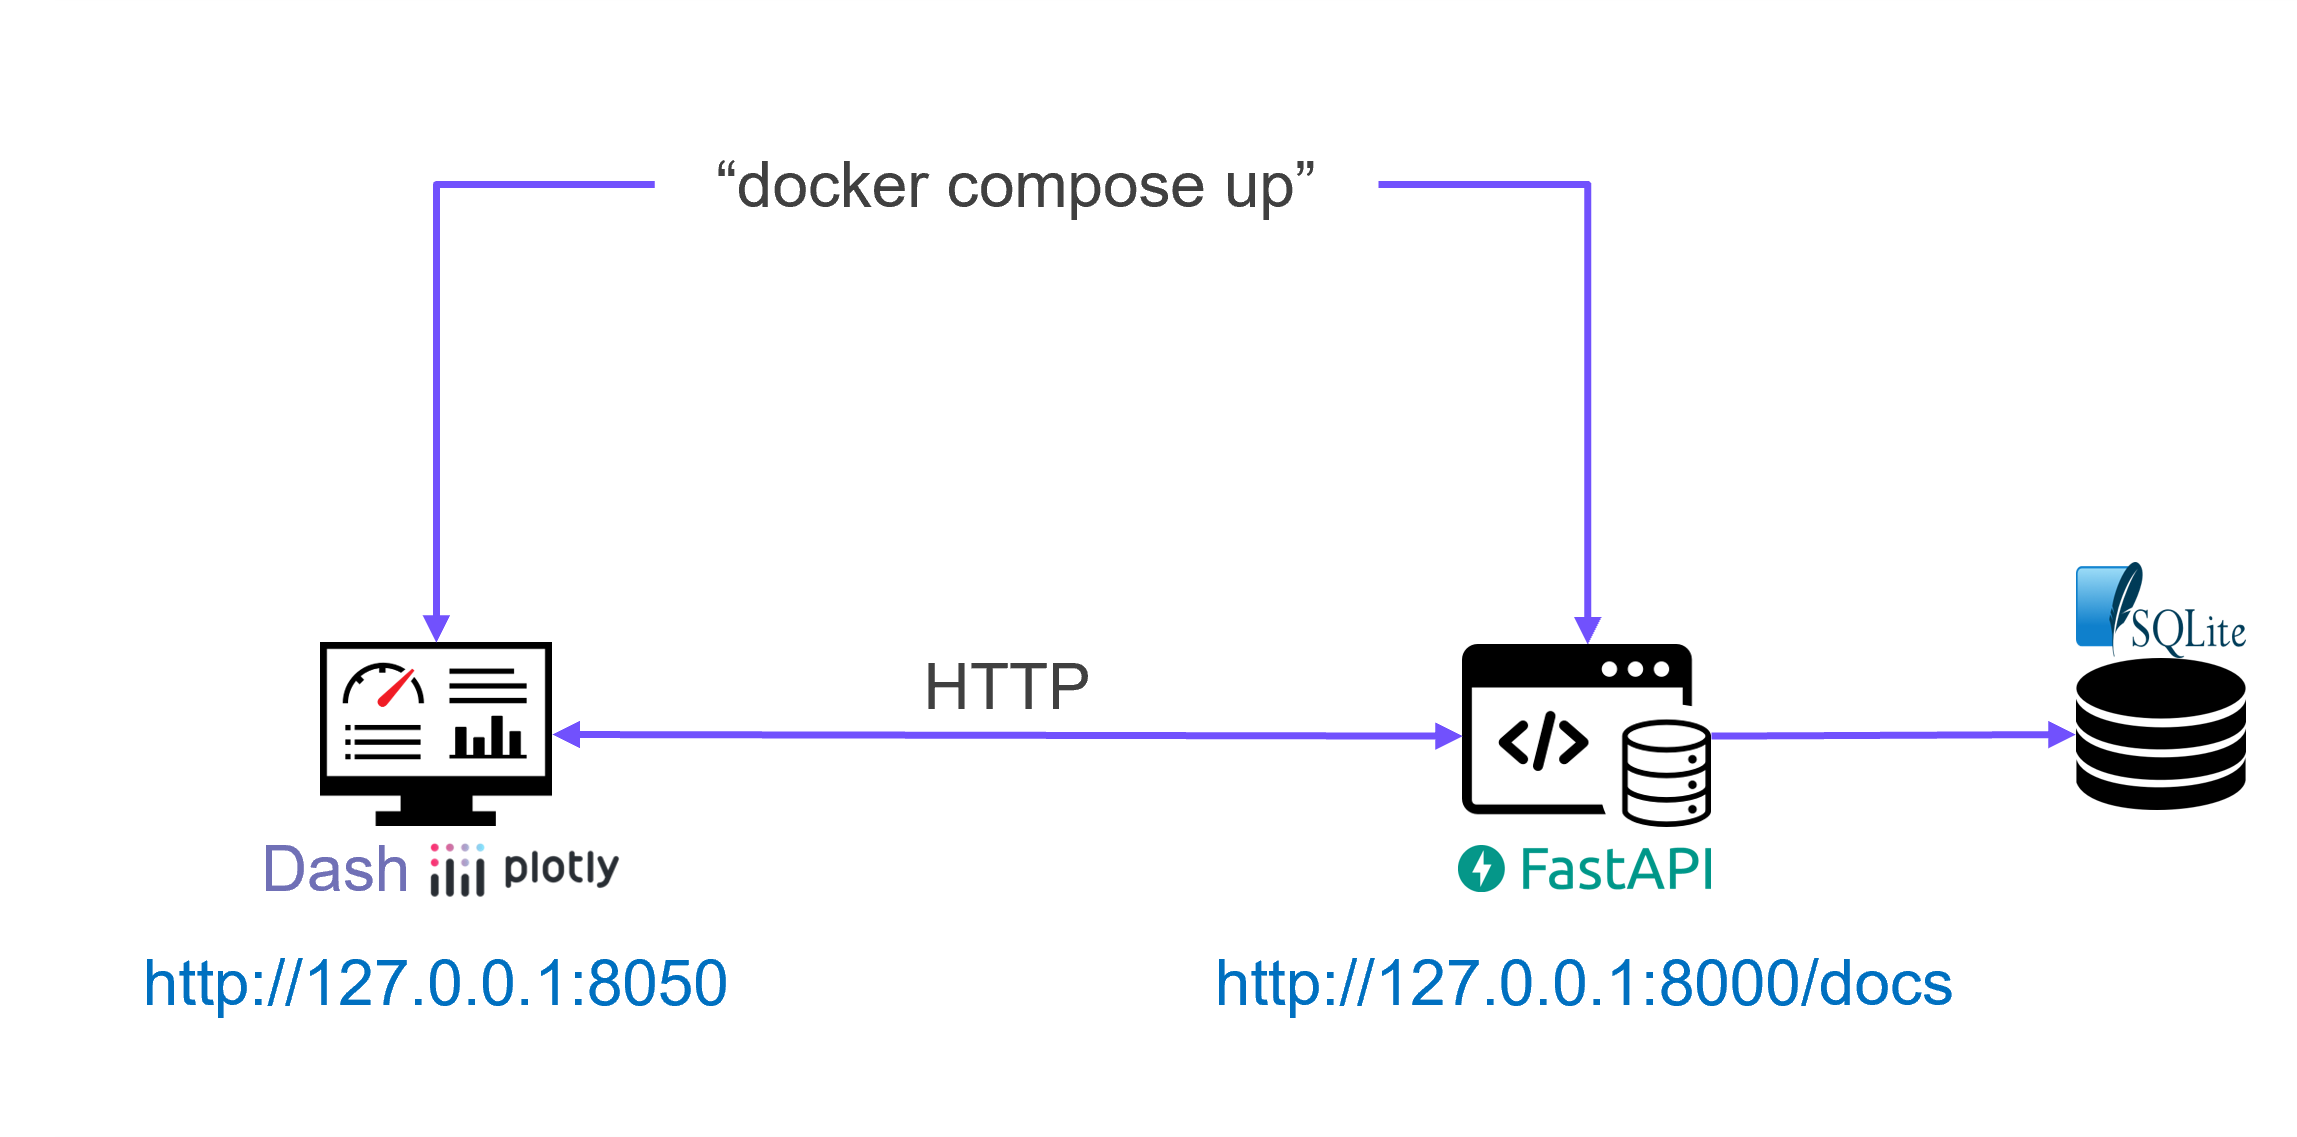
\includegraphics[
	width=\textwidth,
	height=0.75\textheight,
	keepaspectratio
	]{docker-deployment.png}
	\caption{Containerised deployment and communication between services.}
	\label{fig:docker-deployment}
\end{figure}

Introduce the relevant services:

PostgreSQL;
backend;
frontend;
data update;
Airflow;
Prometheus;
Pushgateway;
Alertmanager;
Grafana.

The Docker deployment diagram belongs here.

\subsection{Persistent Storage and Service Dependencies}
PostgreSQL volume;
generated-data volume;
Grafana and Prometheus volumes;
PostgreSQL health check;
%depends_on;
localhost-only port bindings where applicable.

\subsection{ETL Orchestration with Airflow}
Describe:

the Extract, Transform, and Load tasks;
task dependencies;
daily execution at 06:00;
catchup=False;
the Airflow Docker service.

\subsection{Manual Operation}
Briefly mention:

%./docker_start.sh
%./docker_update_data.sh --keyword "Data Engineer" --keyword "AI Engineer"

Do not turn this section into a second README.

Approximately 2–2.5 pages.


\section{Monitoring, Reliability and Testing}

\subsection{Monitoring Architecture}

The monitoring architecture is shown in
Figure~\ref{fig:monitoring-architecture}. Long-running services are
scraped directly, whereas the periodic ETL process publishes its
metrics through Pushgateway.

\begin{figure}[htbp]
	\centering
	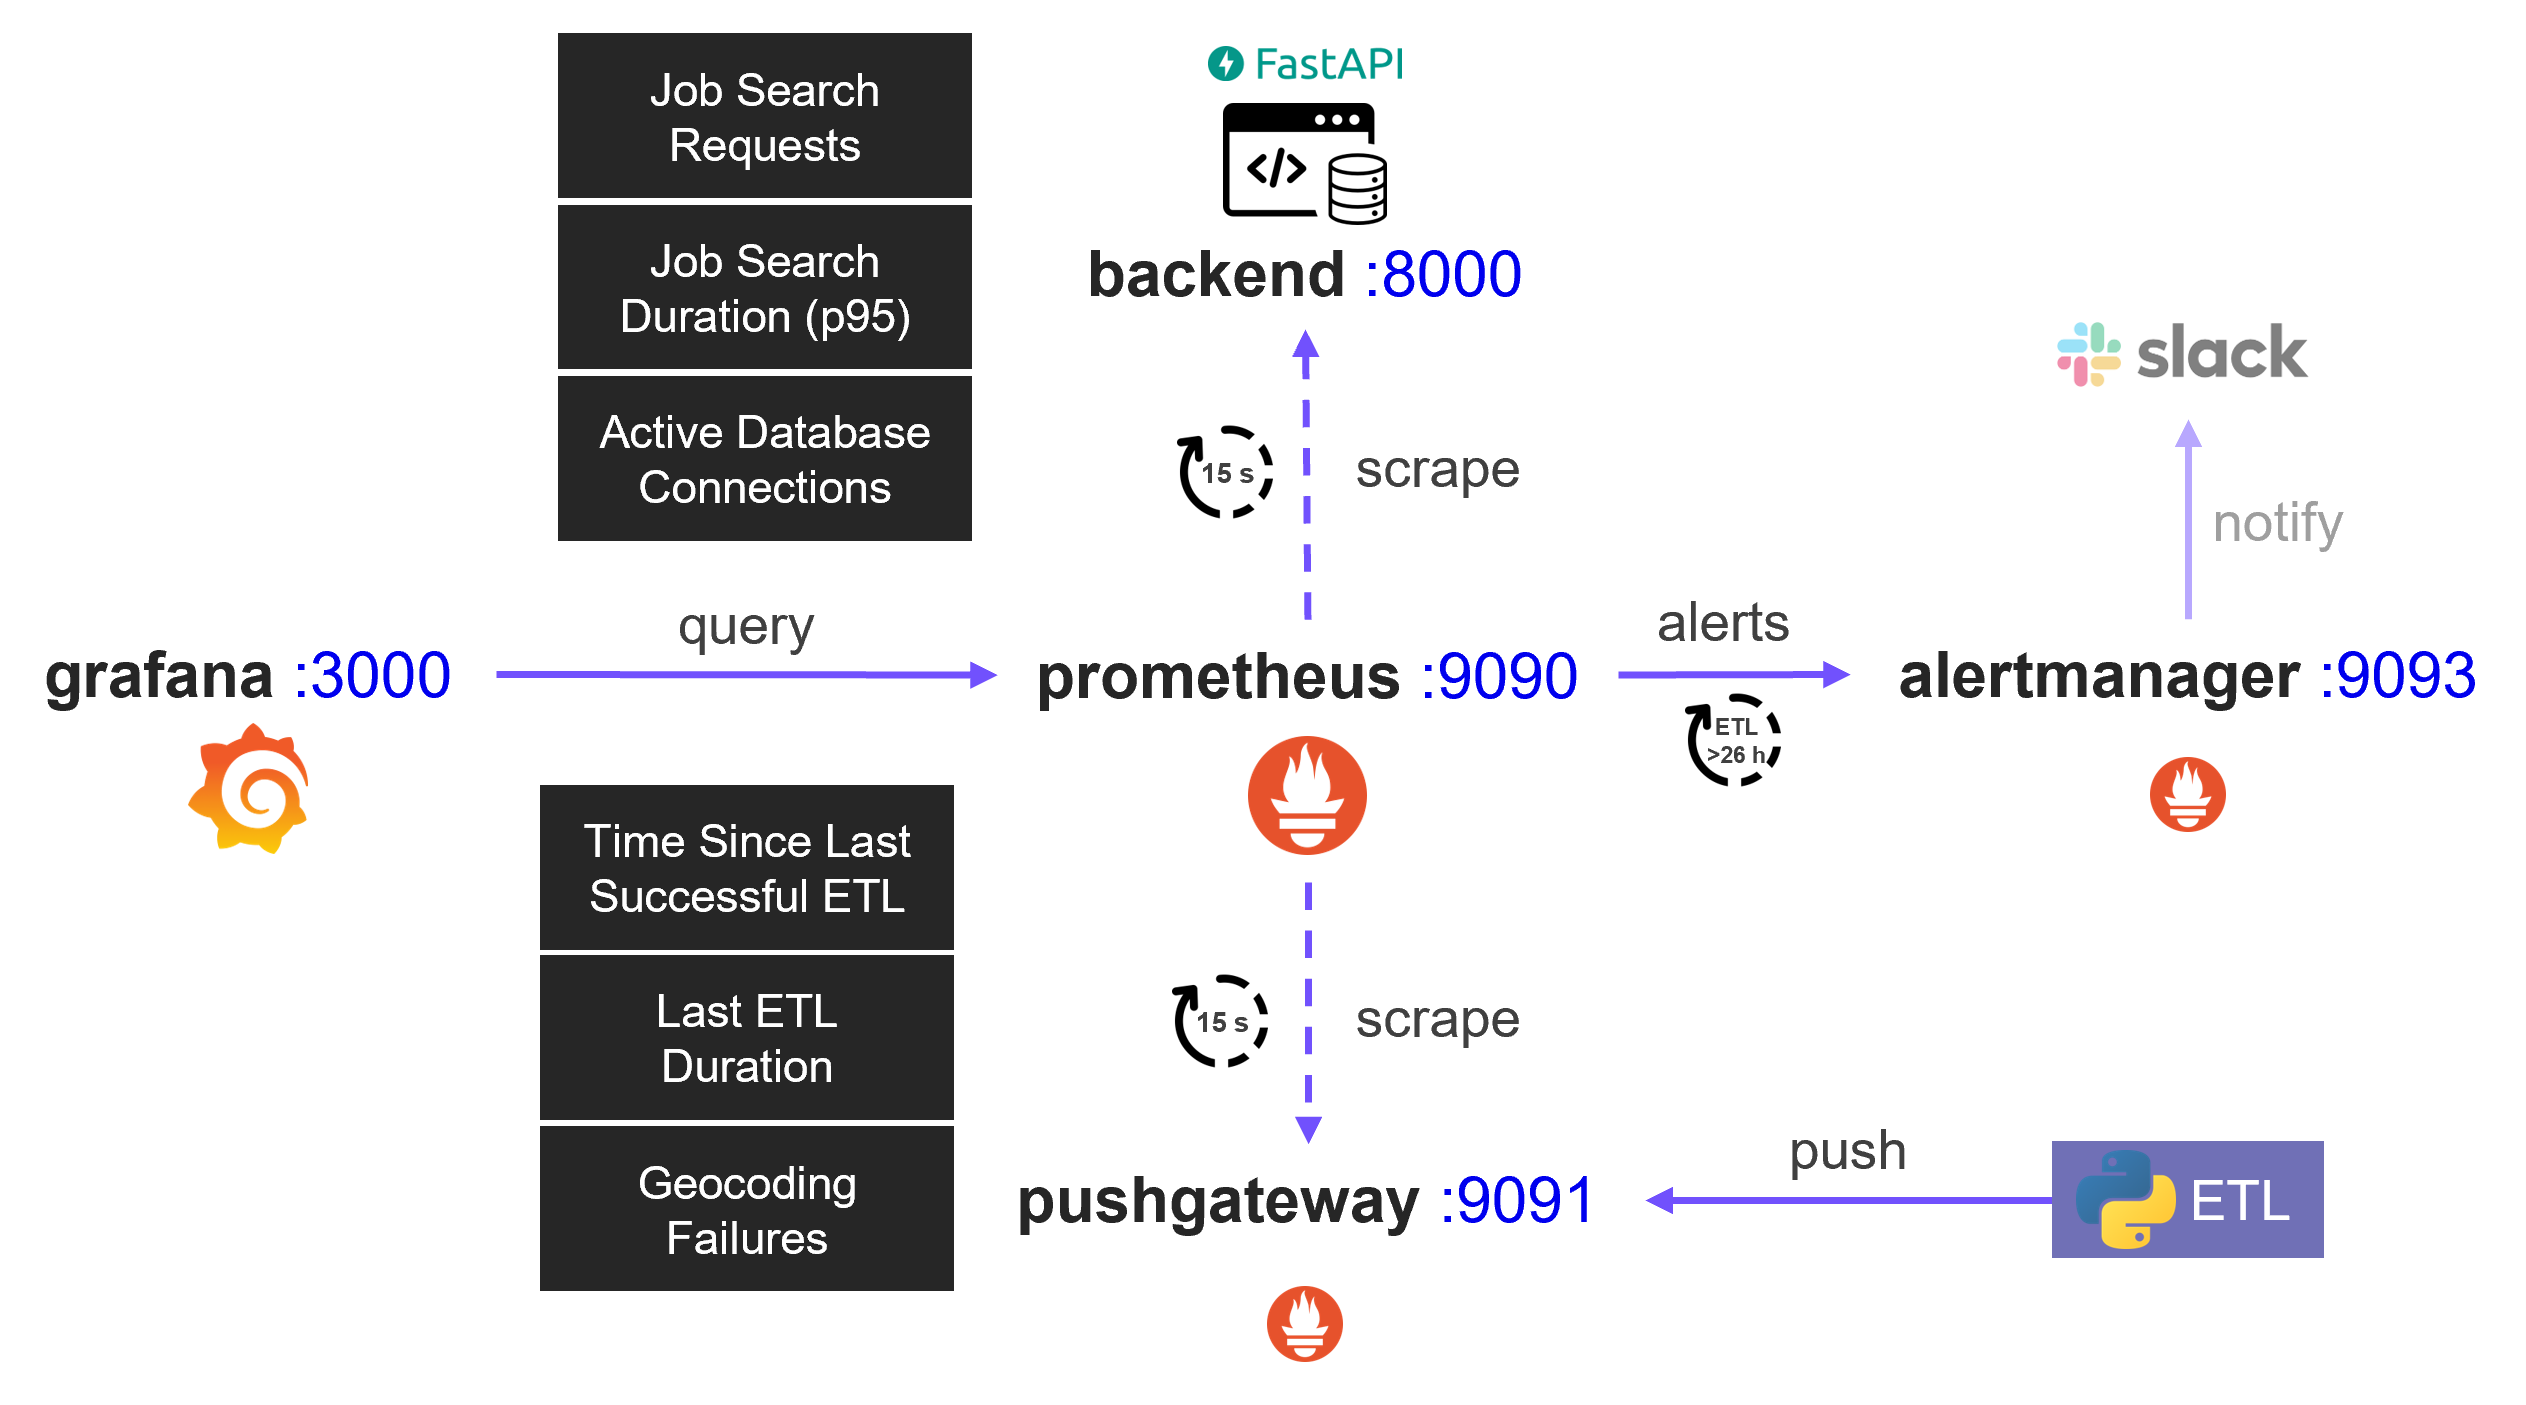
\includegraphics[
	width=\textwidth,
	height=0.75\textheight,
	keepaspectratio
	]{monitoring.png}
	\caption{Monitoring architecture using Prometheus, Pushgateway,
		Grafana, and Alertmanager.}
	\label{fig:monitoring-architecture}
\end{figure}

Explain the roles of:

application metrics;
Prometheus;
Pushgateway;
Grafana;
Alertmanager.

The monitoring diagram belongs here.

\subsection{Collected Metrics}
Group them by component:

Bundesagentur API availability and request duration;
active database connections;
job-search count and duration;
ETL runtime and last-success timestamp;
failed geocoding requests.

Figure~\ref{fig:grafana-dashboard} shows the Grafana dashboard used to inspect the collected API, database, and ETL metrics.

\begin{figure}[htbp]
	\centering
	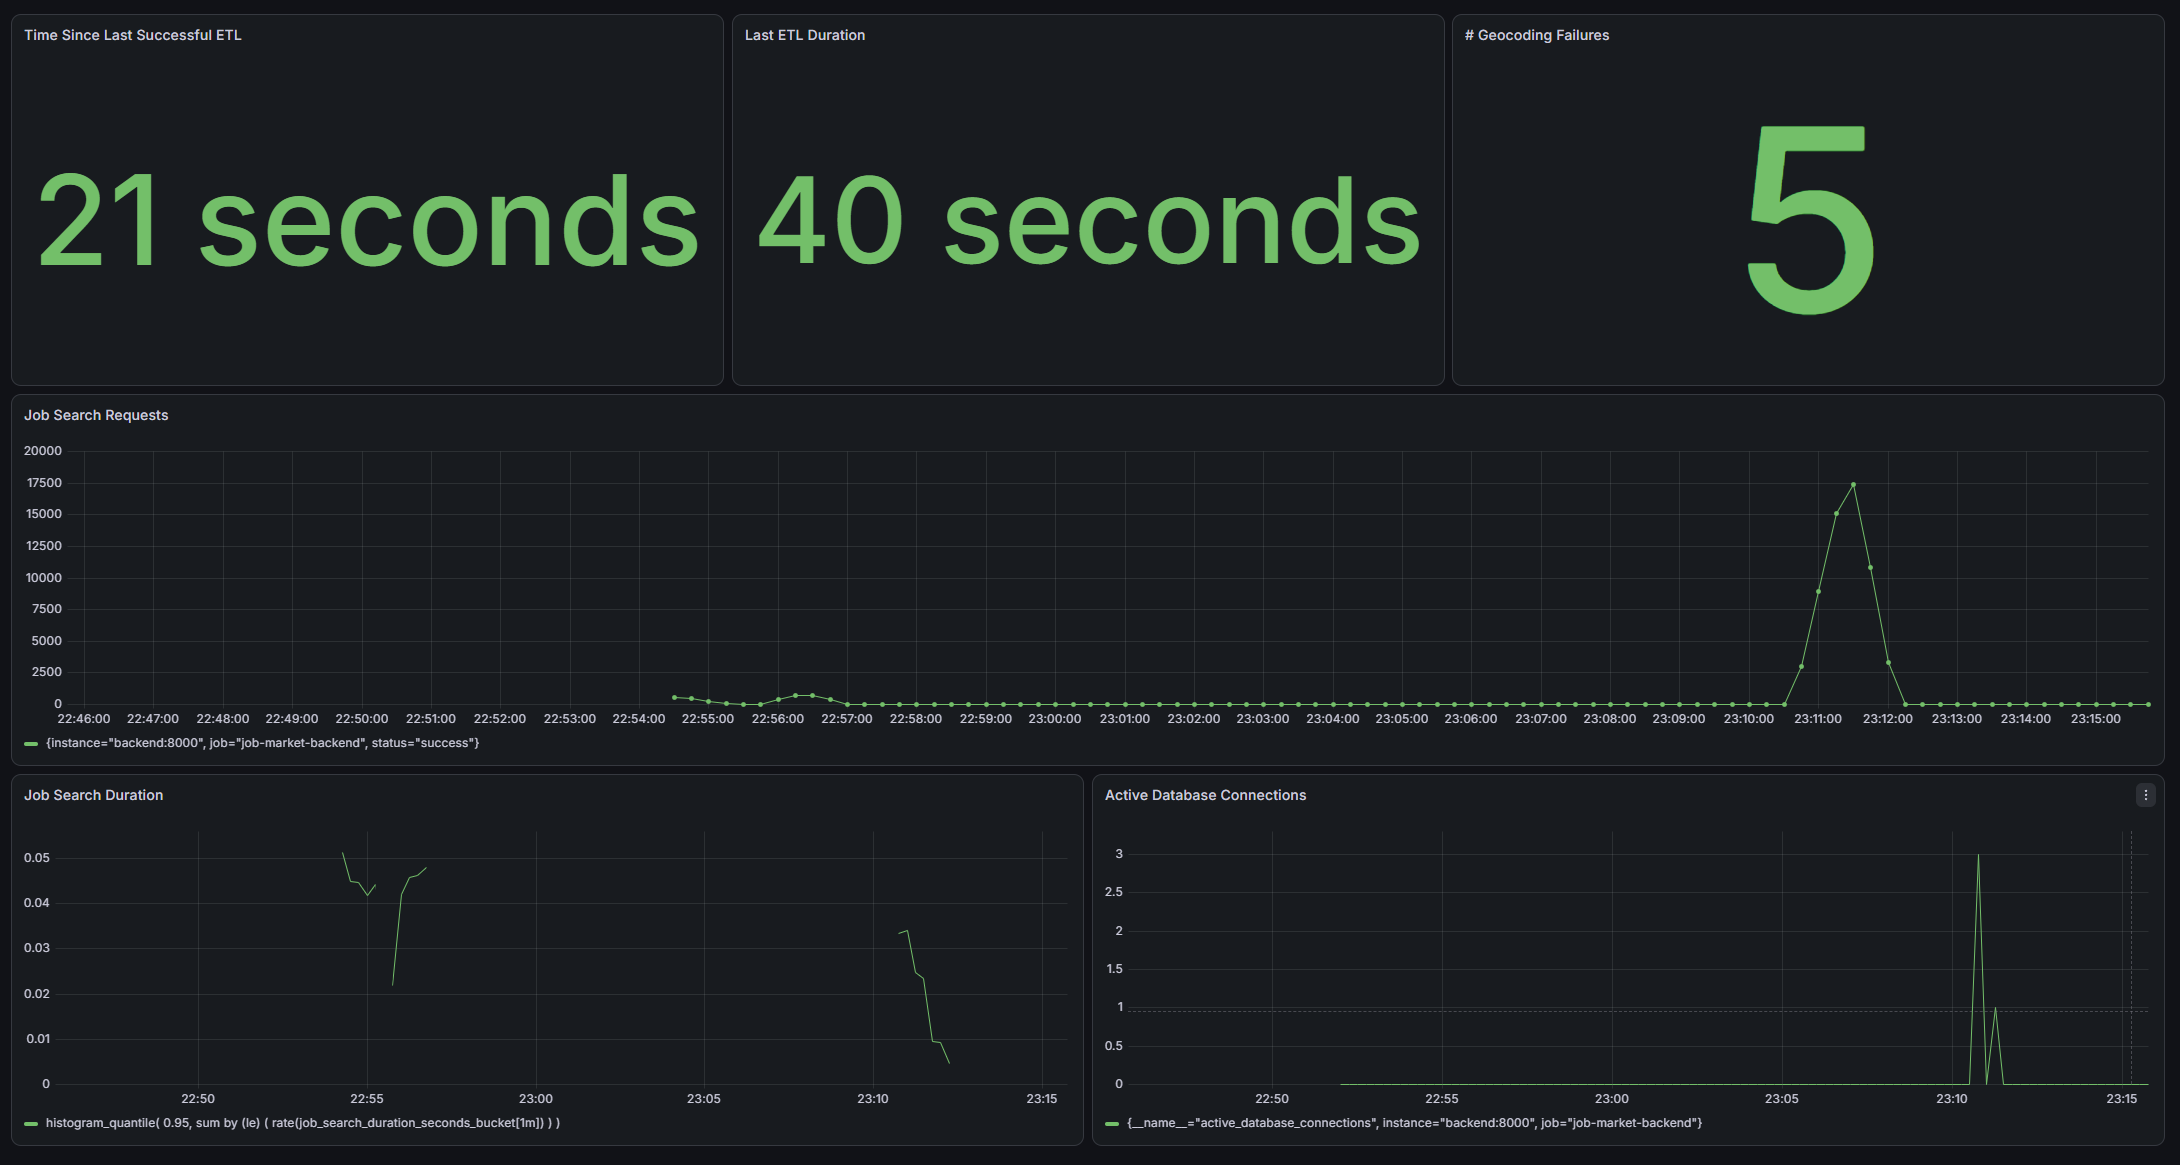
\includegraphics[
	width=\textwidth,
	height=0.58\textheight,
	keepaspectratio
	]{grafana-screenshot.png}
	\caption{Grafana dashboard displaying ETL status, geocoding failures, job-search activity, request duration, and active database connections.}
	\label{fig:grafana-dashboard}
\end{figure}

The upper panels report the freshness and duration of the latest ETL run and the number of geocoding failures. The time-series panels show job-search activity, request duration, and active database connections. The values in Figure~\ref{fig:grafana-dashboard} represent one observed local test run. They demonstrate that the metrics are collected and visualized, but should not be interpreted as a general performance benchmark.

\subsection{Monitoring Periodic ETL Jobs}
Explain specifically why Pushgateway is required: the ETL process terminates after running and therefore cannot be scraped continuously like FastAPI.

\subsection{Error Handling}
Mention:

failed API requests;
failed job-detail extraction;
unavailable PostgreSQL;
HTTP 503 responses;
dashboard notification;
geocoding failures;
ETL monitoring.	

\subsection{Automated Tests and Continuous Integration}
Be honest about the current implementation:

category-classification tests;
short-keyword boundary test;
classification-priority test;
smoke test;
planned GitHub Actions checks: Black, pytest, and Docker image build.

If CI is implemented before submission, describe it as completed. Otherwise, clearly identify it as planned work.

Approximately 1.5–2 pages.

\section{Results and Evaluation}


\subsection{Achieved Results}
Summarise what the complete system can demonstrably do.

\subsection{Technical Decisions}

PostgreSQL was preferred over using JSON as the application database because the transformed data is relational and must support reliable, efficient filtering, joins, and aggregation.

Evaluate the important choices:


FastAPI as the access layer;
Dash as the frontend;
separate raw and processed data;
Docker Compose for reproducibility;
Airflow for scheduling;
Prometheus and Grafana for operational visibility.

\subsection{Limitations}
Mention genuine limitations:

only one job-data source;
rule-based category classification;
keyword search currently based on SQL LIKE;
geocoding depends on an external service;
limited automated test coverage;
deployment intended primarily for a local environment;
no authentication or public production deployment.

\subsection{Possible Improvements}
Potential improvements:

Elasticsearch full-text search and relevance ranking;
job-publication trends;
tracking modified, disappeared, and republished advertisements;
expanded tests;
completed CI pipeline;
additional data sources;
improved classification.

Approximately 1.5 pages.


\section{Conclusion}
A concise final assessment:

what was built;
whether the objectives were achieved;
what the project demonstrates about data-engineering skills;
the most important lesson or outcome.

Approximately half a page.


\printbibliography[heading=bibintoc, title={References}]

\end{document}


%References
%Bundesagentur für Arbeit API;
%FastAPI;
%Dash;
%PostgreSQL;
%SQLAlchemy;
%Docker;
%Airflow;
%Prometheus;
%Grafana;
%Nominatim usage policy.